\section{Experiments}
\label{sec:experiments}
We evaluate the proposed method in two real-robot bimanual expose--execute--restore tasks: the Surgical-Task Setup and the Daily-Task Setup.
In both setups, the robot must retract a deformable occluder to expose the target, 
execute the target-directed manipulation, and restore the occluder.
To evaluate the proposed framework, our experiments study the following questions.
\begin{enumerate}
    \item Can quality-aware iterative annotation produce large-scale, reliable semantic masks with only a few manual annotations?
    \item Does the proposed method improve complete-task performance over the baselines?
    \item Do these improvements generalize across variations in objects, scenes, and spatial configurations?
    \item How do semantic inputs and task-query supervision each contribute to complete-task performance?
\end{enumerate}

\subsection{Experimental Setup}
\label{sec:experimentalsetup}

\subsubsection{Surgical-Task Setup}
The surgical setup (Fig.~\ref{fig:twosettings}a) uses a dual-UR system to manipulate tissue-mimicking material.
One arm retracts the material to establish visibility and access, while the other grasps the exposed target and transfers it to the designated region.
We evaluate four combinations of two target colors and two spatial layouts, with five independently reset trials per condition and 20 trials per policy.
Each trial has a 180-s horizon, and the saved operator-confirmed outcome determines task success.
All policies share the same robot interface, workspace limits, task-specific demonstrations, and right-gripper fallback configuration.

\subsubsection{Daily-Task Setup}
The daily setting (Fig.~\ref{fig:twosettings}b) uses two SO-ARM101 manipulators and fixed front and side cameras with $640\times360$ images.
The 108 demonstrations contain 61,740 synchronized frames recorded at 30 Hz with 10-dimensional joint states and commands.
The demonstrated objects are a cube, paper ball, and screw.
The test set adds a crayon category absent from the policy demonstrations.
For each of the four objects, we test a $4\times3$ grid of initial positions twice, giving 96 trials per policy and 480 trials across five policies.
A trial succeeds when the object is fully inside the goal region and front-view cloth coverage exceeds 0.32 within 40 s.

\begin{figure}[t]
\centering
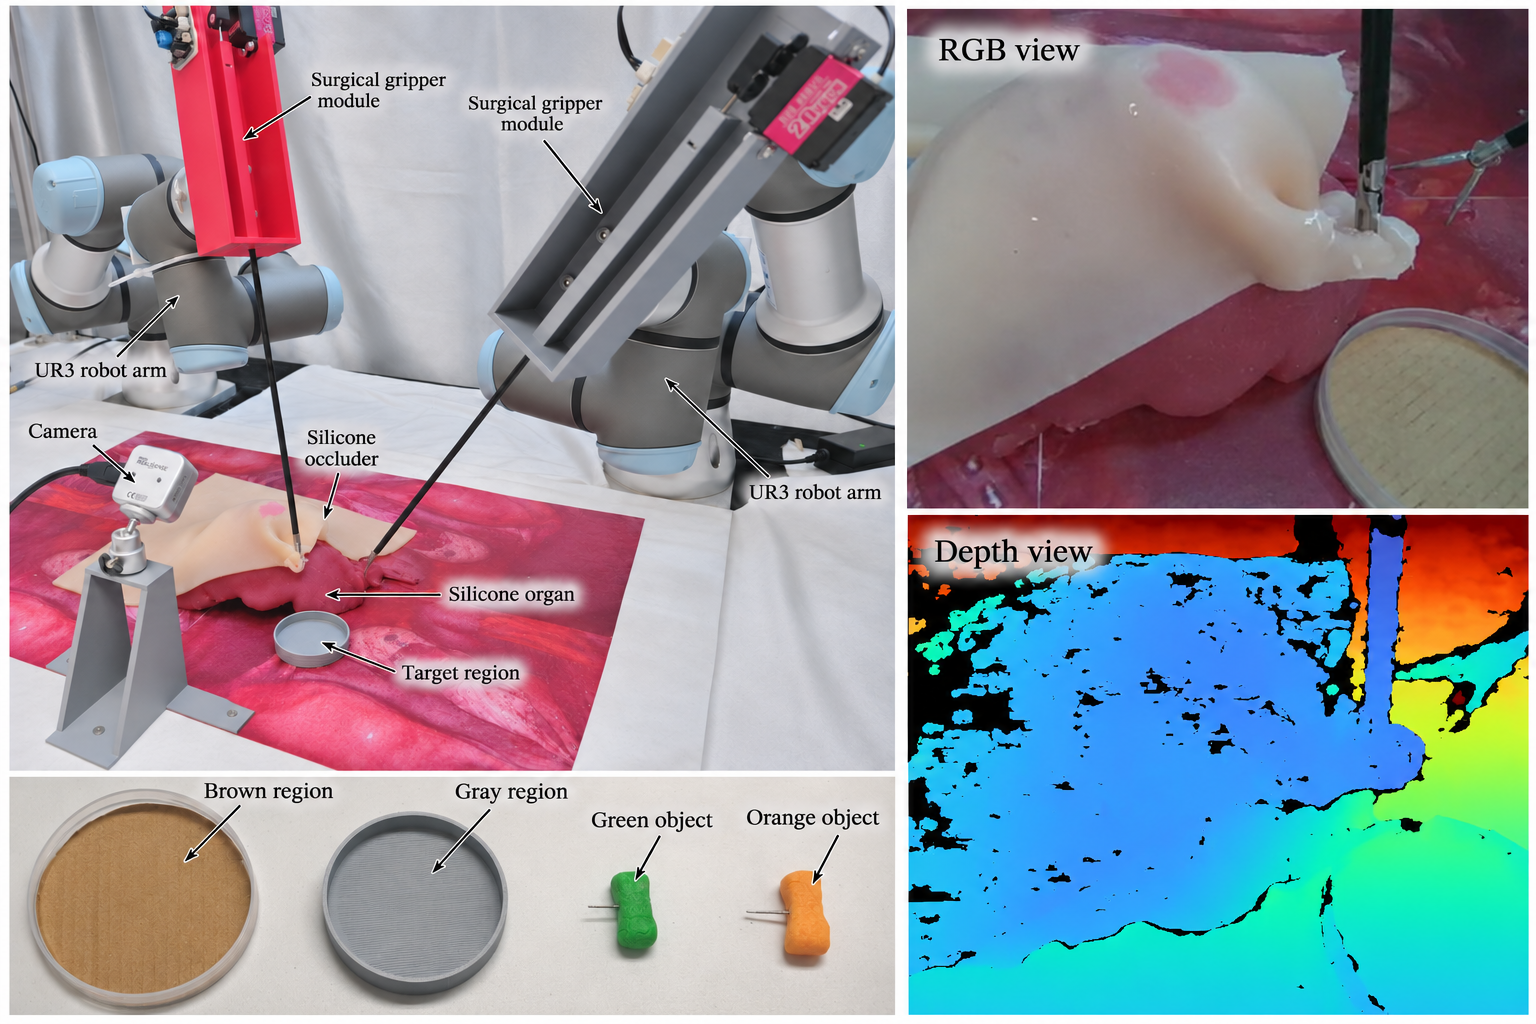
\includegraphics[width=\columnwidth]{myfigure/surgical-task-with-camera-views-v2.png}\par
{\footnotesize (a) Surgical-Task Setup\par}
\vspace{4pt}
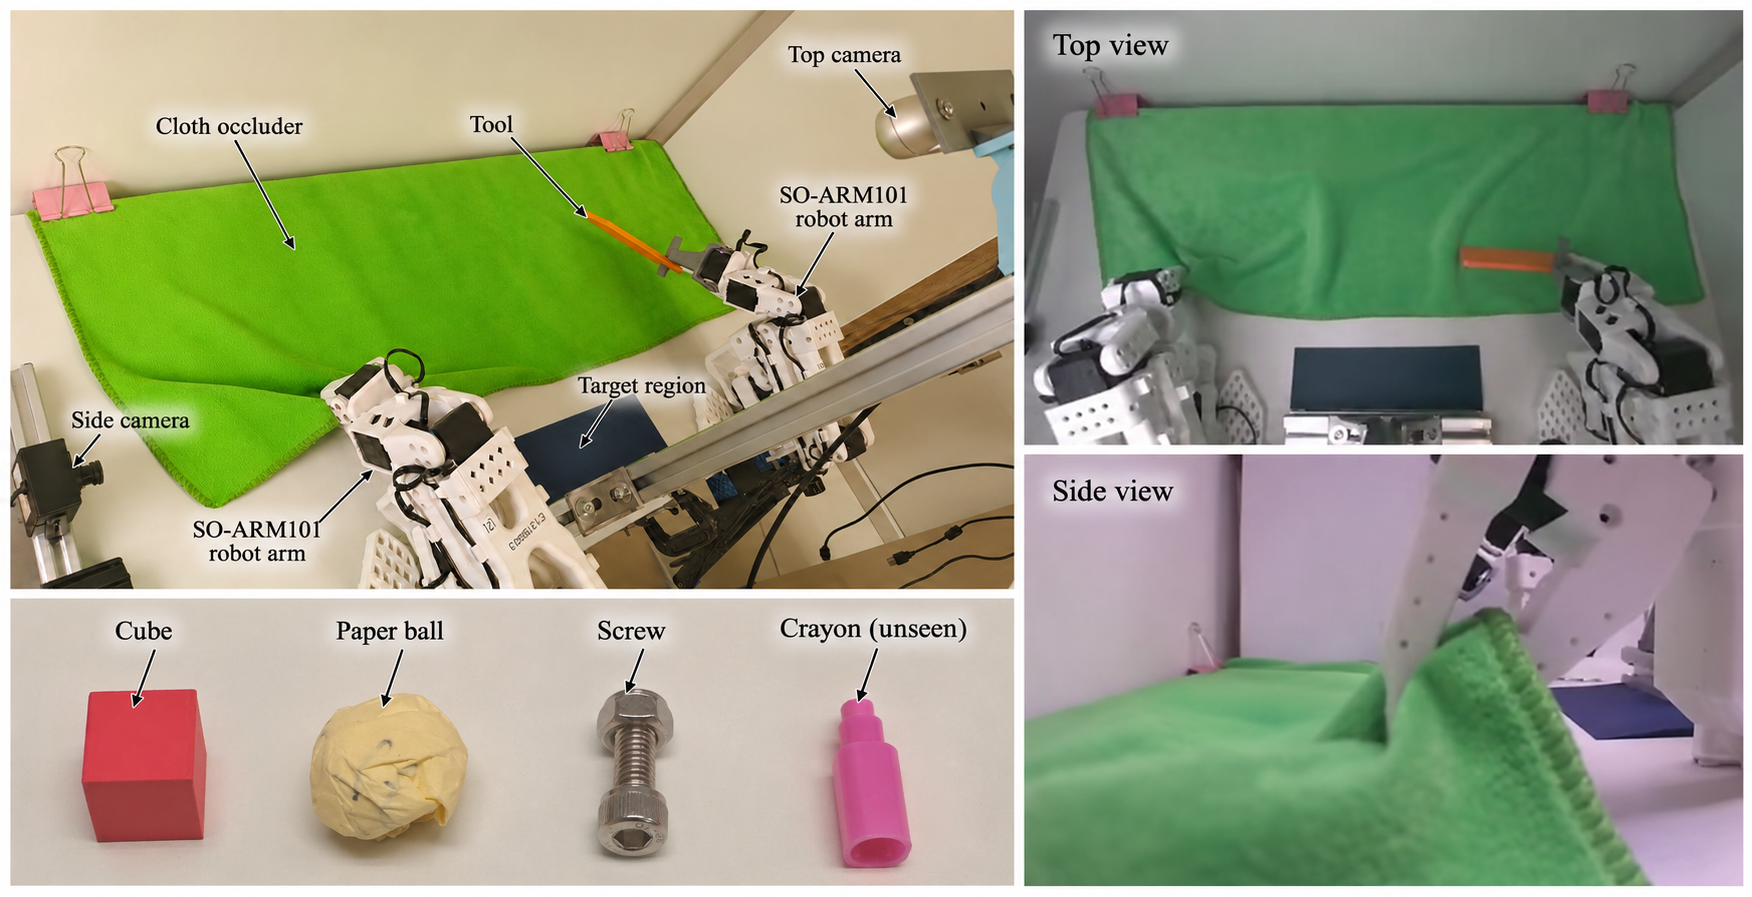
\includegraphics[width=\columnwidth]{myfigure/daily-task-with-camera-views.png}\par
{\footnotesize (b) Daily-Task Setup\par}
\caption{Real-robot experimental setups. (a) Surgical-task setup with two target regions, two colored objects, and RGB and depth views. (b) Daily-task setup with four object categories and top and side views. The crayon category is absent from the policy demonstrations.}
\label{fig:twosettings}
\end{figure}

\subsubsection{Policies and Metrics}
We compare Ours with Action Chunking with Transformers (ACT)~\cite{zhao2023act} and Diffusion Policy (DP)~\cite{chi2023diffusion} in both settings.
The complete task-relation policy is denoted as Ours.
Its controlled variants are named by the removed component: Ours w/o semantic inputs, Ours w/o task-query supervision, and Ours w/o both components, which recovers the ACT backbone.
ACT provides an action-only comparison on the same policy backbone, while DP tests whether an alternative multimodal action-generation objective closes the complete-task gap.
All policies within a setting use the same action demonstrations.
Ours and its controlled variants additionally use the offline semantic supervision specified by their enabled components.

The primary metric is complete-task success.
We also report conditional completion time over successful trials and performance across task conditions, object categories, colors, and initial positions.
Training and deployment configurations are detailed in Appendix~\ref{app:testedimplementation}.

\subsection{Quality-Aware Iterative Annotation}
\label{sec:annotationresults}
\noindent\textbf{Surgical simulation.}
Four reviewed seed videos initialize the front-view segmenter.
Three cumulative generations then train on 8, 24, and 82 quality-screened videos.
A fixed eight-video benchmark contains four anchor videos with reviewed pixel labels and four unseen videos excluded from all training generations.
On the unseen videos, the raw multi-evidence flagged-frame rate decreases from 8.26\% to 3.29\%, while the filtered rate decreases from 2.18\% to 0.54\%.
The anchor foreground mIoU remains stable at approximately 95.4\% across generations, showing that the expansion preserves seed-label agreement while improving temporal and structural consistency on unseen videos.

\begin{table}[t]
\centering
\caption{Surgical-simulation annotation results. Flagged-frame rates decrease on four unseen videos while foreground mIoU remains stable on four reviewed anchor videos.}
\label{tab:surgicalannotation}
\small
\setlength{\tabcolsep}{2.5pt}
\begin{tabular}{lrrrr}
\toprule
Generation & Videos & Raw & Filtered & mIoU\\
\midrule
G1 & 8 & 8.26\% & 2.18\% & 95.45\%\\
G2 & 24 & 6.23\% & 1.12\% & 95.45\%\\
G3 & 82 & 3.29\% & 0.54\% & 95.43\%\\
\bottomrule
\end{tabular}
\end{table}

\noindent\textbf{Daily manipulation.}
Three reviewed seed trajectories train the initial per-view segmenters, and three held-out trajectories track cross-generation performance.
The three cumulative rounds add 15, 29, and 58 new trajectories, yielding 47,766 accepted front-view masks and 42,010 accepted side-view masks in the final pool.

\begin{figure}[t]
\centering
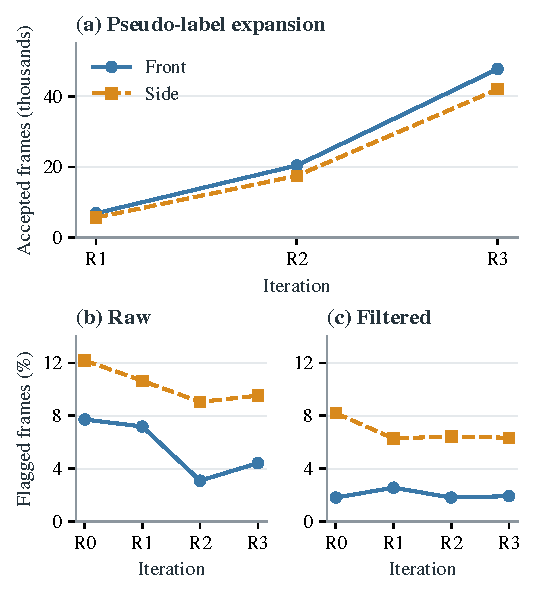
\includegraphics[width=\columnwidth]{figures/annotation_finaldata/annotation_iteration_en.pdf}
\caption{Quality-aware annotation expansion. Accepted supervision increases across rounds, while held-out flagged-frame rates are lower at R3 than at R0 but are not monotonic across rounds.}
\label{fig:annotationiteration}
\end{figure}

On the held-out trajectories, the raw flagged-frame rate decreases from 7.72\% to 4.42\% in the front view and from 12.19\% to 9.53\% in the side view between R0 and R3.
Both views attain their lowest raw rate at R2 rather than R3.
After structural filtering, the side-view rate decreases from 8.20\% to 6.34\%, while the front-view rate changes from 1.81\% to 1.92\%.
The final seed-reference foreground mIoU is 97.87\% for the front view and 97.65\% for the side view.
Across both settings, cumulative self-training expands semantic supervision while maintaining high seed agreement, but increasing the pseudo-label pool does not improve every held-out diagnostic monotonically.

\FloatBarrier

\subsection{Task Evaluation Performance}
\label{sec:overallresults}

\subsubsection{Comparison in the Two Settings}
\noindent\textbf{Surgical simulation.}
Table~\ref{tab:surgicalcomparison} reports results for the two target colors and two spatial layouts.
Ours succeeds in 19 of 20 trials (95.0\%), compared with 8 of 20 (40.0\%) for ACT and 11 of 20 (55.0\%) for DP.
The improvement is consistent across all four evaluated conditions.
Among successful trials, the mean execution time of Ours is 93.12 s, close to ACT at 89.33 s and below DP at 109.62 s.
This conditional comparison evaluates the duration of successful executions rather than overall efficiency across failures.

\begin{table}[t]
\centering
\caption{Surgical-simulation comparison. Ours achieves the highest complete-task success in every color--layout condition. Each condition contains five trials.}
\label{tab:surgicalcomparison}
\small
\setlength{\tabcolsep}{3.2pt}
\begin{tabular}{lccccc}
\toprule
& \multicolumn{2}{c}{Layout A} & \multicolumn{2}{c}{Layout B} & \\
\cmidrule(lr){2-3}\cmidrule(lr){4-5}
Method & Orange & Green & Orange & Green & Overall\\
\midrule
ACT & 2/5 & 1/5 & 2/5 & 3/5 & 8/20\\
DP & 3/5 & 2/5 & 4/5 & 2/5 & 11/20\\
\textbf{Ours} & \textbf{5/5} & \textbf{5/5} & \textbf{5/5} & \textbf{4/5} & \textbf{19/20}\\
\bottomrule
\end{tabular}
\end{table}

\begin{figure}[t]
\centering
\fbox{\parbox{0.92\columnwidth}{\centering\small
\vspace{7pt}
(a) Surgical layout map\\[4pt]
(b) Success by target color and location\\[4pt]
(c) Completion-time distribution
\vspace{7pt}}}
\caption{Condition-level surgical results. The spatial layout, color-wise success, and completion-time plots will replace this placeholder.}
\label{fig:surgicalconditions}
\end{figure}

\noindent\textbf{Daily manipulation.}
Ours succeeds in 92 of 96 trials (95.8\%), improving over ACT and DP by 39.6 and 43.8 percentage points, respectively.
It succeeds in 23 of 24 trials for every object category, including the crayon category absent from the demonstrations.
Among successful trials, its mean completion time is 14.77 s, compared with 14.96 s for ACT and 15.28 s for DP.
When failures are included, the mean control time is 15.82 s for Ours, compared with 25.92 s for ACT and 27.13 s for DP, because most baseline failures reach the 40-s horizon.
This all-trial measure reflects reliability as well as execution speed.
The blocked exact comparisons give Holm-adjusted $p=3.83\times10^{-10}$ against ACT and $p=8.57\times10^{-12}$ against DP.

\begin{table}[t]
\centering
\caption{Daily-manipulation comparison. Ours achieves 23/24 successes in every object category, including the crayon category absent from the policy demonstrations.}
\label{tab:mainresults}
\small
\setlength{\tabcolsep}{3.0pt}
\begin{tabular}{lccccc}
\toprule
Method & Cube & Paper & Screw & Crayon & Overall\\
\midrule
ACT & 18/24 & 12/24 & 11/24 & 13/24 & 54/96\\
DP & 12/24 & 16/24 & 13/24 & 9/24 & 50/96\\
\textbf{Ours} & \textbf{23/24} & \textbf{23/24} & \textbf{23/24} & \textbf{23/24} & \textbf{92/96}\\
\bottomrule
\end{tabular}
\end{table}

Figure~\ref{fig:comparisonpositions} shows the spatial distribution of task success for the comparison methods.
Ours achieves at least 7/8 successes at every grid position, whereas the worst positions of ACT and DP reach only 1/8 and 0/8.
The gains therefore extend across object categories and initial positions rather than concentrating in a small subset of conditions.

\begin{figure}[t]
\centering
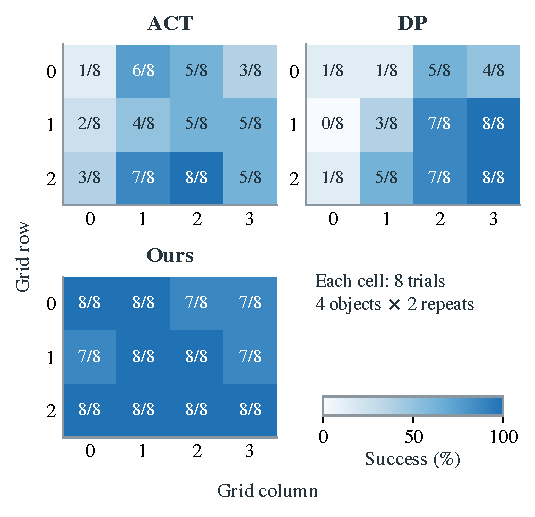
\includegraphics[width=\columnwidth]{figures/results_20261023/position_comparison_en.pdf}
\caption{Spatial comparison in daily manipulation. Ours achieves at least 7/8 successes at every position. Each cell contains eight trials from four objects and two repeats.}
\label{fig:comparisonpositions}
\end{figure}

\subsubsection{Ablation in the Two Settings}
\noindent\textbf{Surgical simulation.}
\draftnote{Insert the surgical ablation results and color--layout analysis.}

\noindent\textbf{Daily manipulation.}
Removing both semantic inputs and task-query supervision gives 54/96 successes.
Retaining only task-query supervision increases success to 72/96, while retaining only semantic inputs gives 60/96.
Combining both components produces the strongest result at 92/96.
Task-query supervision provides the larger standalone gain, increasing success from 54/96 to 72/96 compared with 60/96 from semantic inputs alone.
The larger conditional gains in the combined configurations provide descriptive evidence that the two components are complementary.

\noindent\textbf{Failure-stage analysis.}
ACT and DP leave 34 and 43 trials, respectively, in the separated-but-not-in-region category, compared with 19 for Ours w/o semantics, 31 for Ours w/o task queries, and 4 for Ours.
These labels describe the furthest observed task stage rather than the cause of failure, but show that the main improvement occurs when converting successful exposure and separation into complete transfer.

\begin{figure}[t]
\centering
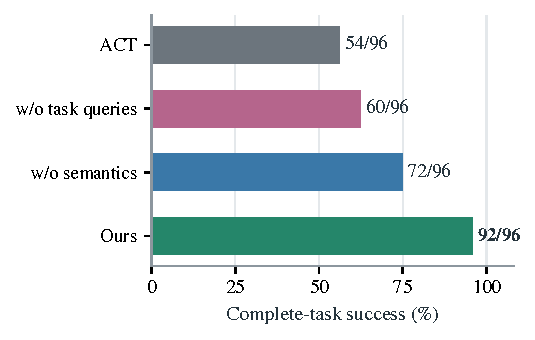
\includegraphics[width=\columnwidth]{figures/results_20261023/ablation_en.pdf}
\caption{Daily-manipulation factorial ablation. Task-query supervision provides the larger standalone gain, while combining both components yields the highest success.}
\label{fig:dailyablation}
\end{figure}
